%!TEX root = ../book.tex
\chapter{Kinematics}\label{chap:kinematics}

In order to plan a robot's movements, we have to understand the relationship between our control variables (i.e. the input to the motors that we can control at any given time) and the effect of these control variables on the motion of the robot.
The simplest models of such relationships can be built by looking at the geometry of our robot, known as the field of \textsl{kinematics}\index{Kinematics}.
For simple arms in static configurations, a kinematic model is rather straightforward: if we know the generalized position / configuration angle of each joint, we can calculate the generalized position of its end-effectors using trigonometry---a process known as \textsl{forward kinematics}\index{Forward Kinematics}.
A more interesting, useful, and complex problem is trying to compute the inverse relationship, i.e. the position each joint needs to be at in order for the end-effector to be in a desired position or pose. This inverse process is known as \textsl{inverse kinematics}\index{Inverse Kinematics}.
For mobile robots, this process is usually more involved, as the pose of the wheels itself at any given time is not conclusive speeds need to be integrated, which we refer to as \textsl{odometry}\index{Odometry}.

As we will see below, kinematics is the simplest and most fundamental level of abstraction that a roboticist can use to model the motion of a robot and its geometry: it deals exclusively with positional quantities, and considers the robot as if it was frozen in time. Although this simplification is far from being realistic, we will see that a lot can be done through kinematics alone! However, a more expressive tool at our disposal is to do a similar modeling in a second level of abstraction that operates in velocity space; this domain is called \textsl{differential kinematics}\index{Differential Kinematics} and is introduced in \cref{sec:kinematics:diff}.
In all, the goals of this chapter are to:

\begin{itemize}
\item introduce the forward kinematics of simple arms and mobile robots, and understand the concept of holonomy,
\item provide an intuition on the relationship between inverse kinematics and path-planning,
\item become familiar with differential kinematics and the Jacobian technique.
\end{itemize}

Within the scope of a kinematic analysis, the term \textsl{generalized position} or \textsl{generalized configuration}\index{Generalized Position}\index{Generalized Configuration} means ``any position-equivalent quantity needed to describe the element''.
For what concerns joint space, it depends on the type of actuation: a revolute joint imparts a rotational motion around its axis and its configuration is fully described by an angle; a prismatic joint commands a translational motion along its axis and its configuration is represented by a distance.
Conversely, generalized position in task space depends on the specific task; in its most general case, a generalized position equates to the end-effector pose, which is composed of a $3D$ position and a $3D$ orientation---as we will see below.

\begin{mdframed}
\noindent Remember:
configuration space $\equiv$ joint space;
cartesian space $\equiv$ task space.
Forward kinematics maps from joint space to task space, and inverse kinematics does the opposite.
The number of mechanical degrees-of-freedom $n$ (i.e. DoFs in task space) depends on the robot, the number of Cartesian degrees-of-freedom $m$ (i.e. DoFs in task space) depends on the task. In general, $n \neq m$!
\end{mdframed}

%%%%%%%%%%%%%%%%%%%%
%% ACTUAL CONTENT %%
%%%%%%%%%%%%%%%%%%%%

%!TEX root = ../book.tex
\section{Forward Kinematics}\label{sec:kinematics:fwkarm}

Now that we have introduced the notion of local coordinate frames, we are interested in calculating the pose and speed of these coordinate frames as a function of the robot's actuators and joint configuration.
We will first consider simple mechanisms where we can determine the relationship between actuators and the pose of various frames on the robot both in the position and speed domain. We will then consider the special class of non-holonomous mechanisms using a series of wheeled robots, for which the forward kinematics can only be calculated in the speed domain.

\subsection{Forward Kinematics of a simple robot arm}

\begin{figure}[!htb]%{L}{0.3\textwidth}
    \centering
    % 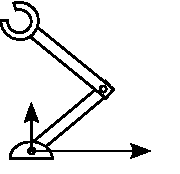
\includegraphics[width=0.27\textwidth]{figs/fwk2dofarm}
    \def\svgwidth{0.4\textwidth}
    \import{./figs/}{fwk2dofarm.pdf_tex}
    \caption{A simple 2-DOF arm.}\label{fig:fwk2dofarm}
\end{figure}

Consider the robot arm in \cref{fig:fwk2dofarm}; it is mounted to a table, and is composed of two links and two joints. Let the length of the first link be $l_1$ and the length of the second link be $l_2$. You could specify the position of the link closer to the table by the angle $\alpha$ and the angle of the second link relative to the first link using the angle $\beta$.

We can now calculate the position $P_1 = (x_1, y_1)$ of the joint between the first and the second link using simple trigonometry:
%
\begin{eqnarray}\label{eq:cosxl1}
x_1 &=&l_1 \cos \alpha \nonumber \\
y_1 &=&l_1 \sin \alpha
\end{eqnarray}
%
Similarly, the position of the end-effector $P_2 = (x_2, y_2)$ is given by:
%
\begin{eqnarray}
x_2&=&x_1 + l_2 \cos(\alpha+\beta) \nonumber \\
y_2&=&y_1 + l_2 \sin(\alpha+\beta)
\end{eqnarray}
%
or together, the position of the end-effector $(x,y)$ is given by
%
\begin{eqnarray}\label{eq:cosx}
x&=&l_1 \cos \alpha + l_2 \cos(\alpha+\beta) \nonumber \\
y&=&l_1 \sin \alpha + l_2 \sin(\alpha+\beta)
\end{eqnarray}
%
The above equations represent \textsl{the forward kinematic equations} of the robot---as they relate its control parameters $ \alpha$ and $\beta$ (also known as joint configuration) to the position of its end-effector in the local coordinate system spanned by $ x$ and $ y$ with the origin at the robot's base.
Note that both $\alpha$ and $\beta$ shown in the figure are positive: both links rotate around the $z-$axis. Using the right-hand rule, the direction of positive angles is defined to be counter-clockwise.

The \emph{configuration space}\index{Configuration space}\index{C-Space (Configuration space)} of the robot---i.e. the set of angles each actuator can be set to---is given by $ 0 < \alpha < \pi $ as it is not supposed to run into the table, and $ -\pi < \beta < \pi$.
The configuration space is given with respect to the robot's joints and allows us to use the forward kinematics equations to calculate the \emph{workspace}\index{Workspace} of the robot, i.e. the physical space it can move to.
This terminology will be identical for mobile robots. An example of configuration and workspace for both a manipulator and a mobile robot is shown in \cref{fig:holonomy}.

As shown in \cref{fig:fwk2dofarm}, the orientation of the arm's end-effector is given by $\alpha+\beta$. We can now write down  a transformation that includes a rotation around the z-axis:
\begin{equation}
\label{eq:2armtrans}
\left[\begin{array}{cccc}cos_{\alpha\beta} & -sin_{\alpha\beta} &  0 & \cos_{\alpha\beta}l_2+\cos\alpha l_1\\
                        sin_{\alpha\beta} & cos_{\alpha\beta} & 0 & \sin_{\alpha\beta}l_2+\sin\alpha l_1\\
                                                0 & 0 & 1 & 0\\
                                                0 & 0 & 0 & 1\end{array}\right]
\end{equation}
The notation $sin_{\alpha\beta}$ and $cos_{\alpha\beta}$ are shorthand for $sin(\alpha+\beta)$ and $cos(\alpha+\beta)$, respectively.

This transformation now allows us to translate from the robot's base to the robot's end-effector as a function of the joint configuration $\alpha$ and $\beta$.
This transformation will be helpful if we want to calculate suitable joint angles in order to reach a certain pose or if we want to convert measurements taken relative to the end-effector back into the base's coordinate system.

\subsection{Forward Kinematics of a Differential Wheels Robot}\label{sec:kinematics:fwkmobile}

Whereas the pose of a robotic manipulator is uniquely defined by its joint angles---which can be made available using encoders in almost real-time, see \cref{sec:sensors:encoders}---this is not the case for a mobile robot.
Here, the encoder values simply refer to wheel orientation and need to be integrated over time in order to assess the robot's position with respect to the worlds frame of reference; as we will later see, this is a great source of uncertainty.
What complicates matters is that for so-called \emph{non-holonomic} systems, it is not sufficient to simply measure the distance that each wheel traveled, but also when each movement was executed.

\begin{figure}
    \small
    \centering
    % 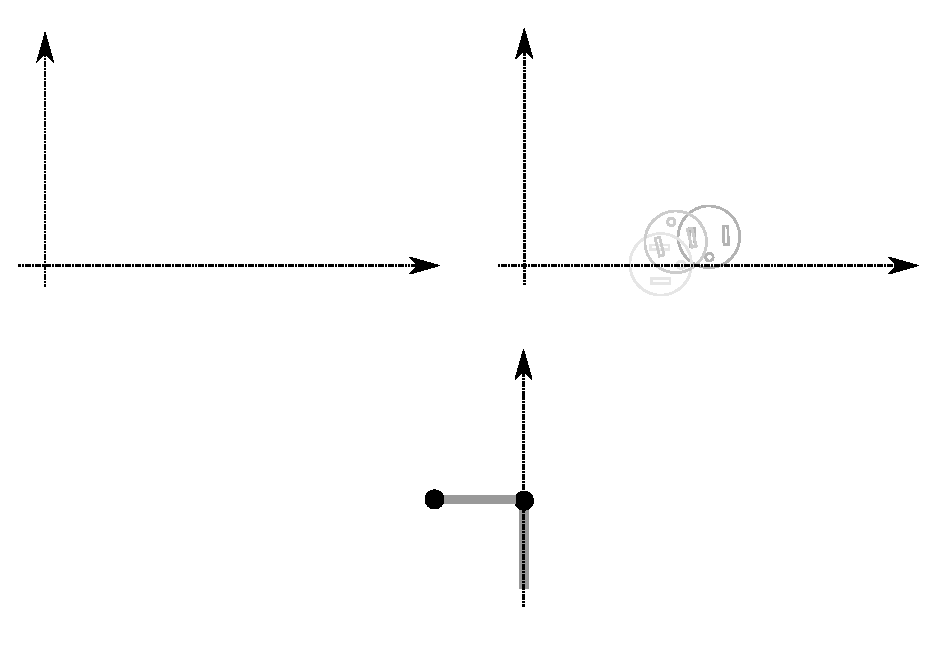
\includegraphics[width=0.95\textwidth]{figs/holonomy.png}
    \def\svgwidth{\textwidth}
    \import{./figs/}{holonomy.pdf_tex}
    \caption{Configuration or joint space (left) and workspace or operational space (right) for a non-holonomic mobile robot (top) and a holonomic manipulator (bottom). Closed trajectories in configuration space result in closed trajectories in the workspace if the robot's kinematics is holonomic.}
    \label{fig:holonomy}
\end{figure}

A system is non-holonomic\index{Non-holonomic}\index{Holonomic} when closed trajectories in its configuration space may not have it return to its original state (reminder: the configuration or joint space space of a two-link robotic arm is spanned by the possible values of each angle).
A simple arm is holonomic because each joint position corresponds to a unique position in space:
going through whatever trajectory that comes back to the starting point in configuration space, will put the robot's end-effector at the exact same position in operational space.
A train on a track is holonomic: moving its wheels backwards by the same amount they have been moving forward brings the train to the exact same position in space.
A car and a differential-wheel robot are non-holonomic vehicles: performing a straight line and then a right-turn leads to the same amount of wheel rotation than doing a right turn first and then going in a straight line; however getting the robot to its initial position requires not only to rewind both wheels by the same amount, but also getting their relative speeds right.
The configuration and corresponding workspace trajectories for a non-holonomic and a holonomic robot are shown in \cref{fig:holonomy}.
Here, a robot first moves on a straight line, i.e. both wheels turn an equal amount.
Then, the left wheel remains fixed and only the right wheel turns forward.
Then, the right wheel remain fixed and the left wheel turns backward.
Finally, the right wheel turns backward, arriving at the initial encoder values (zero).
Yet, the robot does not return to its origin. Performing a similar trajectory in the configuration space of a two-link manipulator instead, lets the robot return to its initial position.

It should be clear by now that for a mobile robot, not only traveled distance per wheel matters, but also the \textsl{speed} of each wheel as a function of time.
Interestingly however, this information was not required to uniquely determine the pose of a manipulating arm.
Let's introduce the following conventions.
We will establish a world coordinate system $\{I\}$---which is known as the inertial frame by convention (see \cref{fig:mobilerobot}).
We establish a coordinate system $\{R\}$ on the robot and express the robot's speed $^R\dot{\xi}$ as a vector $ ^R\dot{\xi}=[^R\dot{x}, ^R\dot{y}, ^R\dot{\theta}]^T$. Here $^R\dot{x}$ and $^R\dot{y}$ correspond to the speed along the $x$ and $y$ directions in $\{R\}$, whereas $^R\dot{\theta}$ corresponds to the rotation velocity around the $z-$axis, that you can imagine to be sticking out of the ground.
We denote speeds with dots over the variable name, as speed is simply the derivative of distance.
Now, let's think about the robot's position in $\{R\}$. It is always zero, as the coordinate system is fixed on the robot itself.
Therefore, velocities are the only interesting quantities in this coordinate system and we need to understand how velocities in $\{R\}$ map to positions in $\{I\}$, which we denote by $^I\xi=[^Ix, ^Iy, ^I\theta]^T$. These coordinate systems are shown in \cref{fig:mobilerobot}.

\begin{figure}[htb!]
    \centering
    % 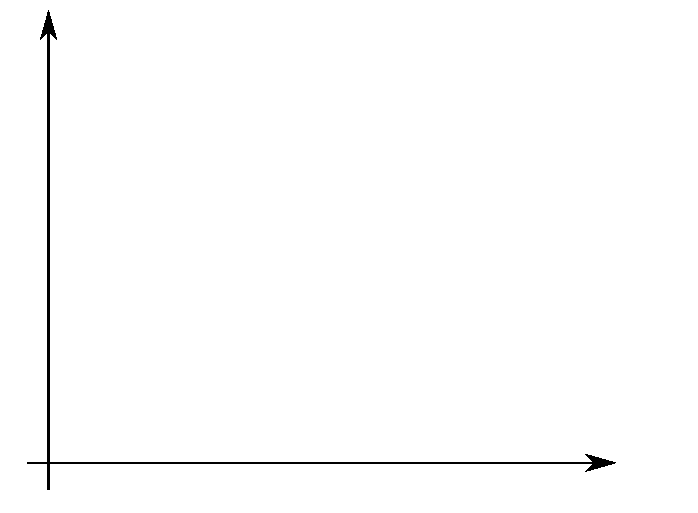
\includegraphics[width=0.85\textwidth]{figs/mobilerobot.png}
    \def\svgwidth{0.85\textwidth}
    \import{./figs/}{mobilerobot.pdf_tex}
    \caption{Mobile robot with local coordinate system \{R\} and world frame \{I\}. The arrows indicate the positive direction of position and orientation vectors.
    \td{Nikolaus: $\theta_i$ in this figure should point downwards right? }}
    \label{fig:mobilerobot}
\end{figure}



Notice that the positioning of the coordinate frames and their orientation are arbitrary. Here, we choose to place the coordinate system in the center of the robot's axle and align $^Rx$ with its default driving direction.
In order to calculate the robot's position in the inertial frame, we need to first find out how speed in the robot coordinate frame maps to speed in the inertial frame.
This can be done again by employing trigonometry. There is only one complication: a movement into the robot's $x-$axis might lead to movement along both the $x-$axis and the $y-$axis of the world coordinate frame ${I}$. By looking at \cref{fig:mobilerobot}, we can derive the following components to $\dot{x}_I$. First,
\begin{equation}
\dot{x}_{I,x}=cos(\theta) \dot{x}_R.
\end{equation}

There is also a component of motion coming from $ \dot{y}_R$ (ignoring the kinematic constraints for now, see below).  For negative $ \theta$, as in \cref{fig:mobilerobot}, a move along $y_R$ would let the robot move into positive $ X_I$ direction. The projection from $ \dot{y}_R$ is therefore given by
\begin{equation}
\dot{x_{I,y}}=-sin(\theta)\dot{y_R}.
\end{equation}
We can now write
\begin{equation}
\dot{x_I}=cos(\theta) \dot{x_R} - sin(\theta) \dot{y_R}.
\end{equation}
Similar reasoning leads to:
\begin{equation}
\dot{y_I}=sin(\theta) \dot{x_R} + cos(\theta) \dot{y_R}
\end{equation}
and
\begin{equation}
\dot{\theta_I}=\dot{\theta_R}
\end{equation}
which is the case because both robot's and world coordinate system share the same z-axis in this example. We can now conveniently write
\begin{equation}
\dot{\xi_I}=^I_RT(\theta)\dot{\xi_R}
\end{equation}
with
\begin{equation}
^I_RT(\theta)=\left[\begin{array}{ccc}
cos(\theta) & -sin(\theta) & 0 \\
sin(\theta) & cos(\theta) & 0 \\
0 & 0 & 1\end{array}\right]
\end{equation}

We are now left with the problem of how to calculate the speed $ \dot{\xi_R}$ in robot coordinates. For this, we make use of the \emph{kinematic constraints}\index{Kinematic constraints} of the robotic wheels.
For a standard wheel in an ideal case scenario, the kinematic constraints are that every rotation of the wheel leads to strictly forward or backward motion and does not allow side-way motion or sliding. We can therefore calculate the forward speed of a wheel $ \dot{x}$ using its rotational speed $ \dot{\phi}$ (assuming the encoder value/angle is expressed as $ \phi$) and radius $ r$ by
\begin{equation}
\dot{x}=\dot{\phi}r.
\end{equation}
This becomes apparent when considering that the circumference of a wheel with radius $r$ is $2\pi r$. The distance a wheel rolls when turned by the angle $ \phi$ (in radians) is therefore $ x=\phi r$, see also \cref{fig:wheelrotation}, right. Taking the derivative of this expression on both sides leads to the above expression.

\begin{figure}[htb!]
    \centering
    % 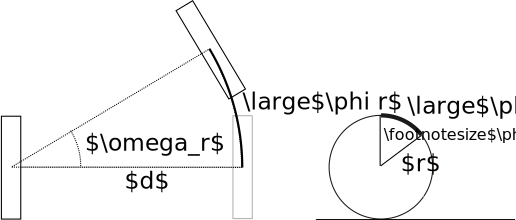
\includegraphics[width=0.9\textwidth]{figs/wheelrotation.png}
    \def\svgwidth{0.86\textwidth}
    \import{./figs/}{wheelrotation.pdf_tex}
    \caption{Left: Differential wheel robot pivoting around its left wheel. Right: A wheel with radius $r$ moves by $\phi r$ when rotated by $\phi$ degrees.}
    \label{fig:wheelrotation}
\end{figure}



How each of the two wheels in our example contributes to the speed of the robot's center---where its coordinate system is anchored---requires the following trick: we calculate the contribution of each individual wheel while assuming all other wheels remaining un-actuated.
In this example, the distance traveled by the center point is exactly half of that traveled by each individual wheel, assuming the non-actuated wheel rotating around its ground contact point (\cref{fig:wheelrotation}). We can therefore write:
\begin{equation}
\dot{x_R}=\frac{r\dot{\phi_l}}{2}+\frac{r\dot{\phi_r}}{2}
\end{equation}
given the speeds $ \dot{\phi_l}$ and $ \dot{\phi_r}$ of the left and the right wheel, respectively.

\begin{framed}
Think about how the robot's speed along its y-axis is affected by the wheel speed given the coordinate system in the drawing above. Think about the kinematic constraints that the standard wheels impose.
\end{framed}

Hard to believe at first, but the speed of the robot along its y-axis is always zero. This is because the constraints of the standard wheel tell us that the robot can never slide.
We are now left with calculating the rotation of the robot around its z-axis.
\td{This sentence is unclear: That there is such a thing can be immediately seen when imaging the robot's wheels spinning in opposite directions}.
We will again consider each wheel independently. Assuming the left wheel to be non-actuated, spinning the right wheel forwards will lead to counter-clockwise rotation. Given an axle diameter (distance between the robot's wheels) $d$, we can now write
\begin{equation}
\omega_r d = \phi_r r
\end{equation}
with $\omega_r$ the angle of rotation around the left wheel (\cref{fig:wheelrotation}, left). Taking the derivative on both sides yields speeds and we can write
\begin{equation}
\dot{\omega_r} = \frac{\dot{\phi_r} r}{d}
\end{equation}
Adding the rotation speeds up (with the one around the right wheel being negative based on the right-hand grip rule), leads to:
%
\begin{equation}
\dot{\theta}=\frac{\dot{\phi_r} r}{d}-\frac{\dot{\phi_l} r}{d}
\end{equation}
%
Putting it all together, we can finally write:

\begin{equation}\label{eq:diffwheels}
\left[\begin{array}{c} \dot{x_I}\\\dot{y_I}\\\dot{\theta}\end{array}\right]=\left[\begin{array}{ccc}
cos(\theta) & -sin(\theta) & 0 \\
sin(\theta) & cos(\theta) & 0 \\
0 & 0 & 1\end{array}\right]\left[\begin{array}{c}\frac{r\dot{\phi_l}}{2}+\frac{r\dot{\phi_r}}{2}\\0\\\frac{\dot{\phi_r} r}{d}-\frac{\dot{\phi_l} r}{d}\end{array}\right]
\end{equation}

\subsubsection{From Forward Kinematics to Odometry}

\cref{eq:diffwheels} only provides us with the relationship between the robot's wheel speed and its speed in the inertial frame.
Calculating its actual pose in the inertial frame is known as \emph{odometry}\index{Odometry}. Technically, it requires integrating \cref{eq:diffwheels} from 0 to the current time $T$.
As this is not possible but for very special cases, one can approximate the robot's pose by summing up speeds over discrete time intervals, or more precisely:
\begin{equation}
\left[\begin{array}{c} {x_I}(T)\\{y_I}(T)\\{\theta}(T)\end{array}\right]=
\int_0^T \left[\begin{array}{c} \dot{x_I}(t)\\\dot{y_I}(t)\\\dot{\theta}(t)\end{array}\right] dt \approx
\sum_{k=0}^{k=T}\left[\begin{array}{c} \Delta{x_I}(k)\\\Delta{y_I}(k)\\\Delta{\theta}(k)\end{array}\right]\Delta t
\end{equation} which can be calculated incrementally as
\begin{equation}\label{eq:odometry}
x_I(k+1)=x_I(k)+\Delta x (k) \Delta t
\end{equation}
using $\Delta x(k) \approx \dot{x_I}(t)$ and similar expressions for $y_I$ and $\theta$. Note that \cref{eq:odometry} is just an approximation. The larger $\Delta t$ becomes, the more inaccurate this approximation becomes as the robot's speed might change during the interval.

\begin{framed}
\noindent Don't let the notion of an integral worry you! As robots' computers are fundamentally discrete, integrals usually turn into sums, which are nothing than for-loops.
\end{framed}

\subsection{Forward kinematics of Car-like steering}\label{sec:kinematics:carsteering}

Differential wheel drives are very popular in mobile robotics as they are very easy to build, maintain, and control.
Although not holonomic, a differential drive can approximate the function of a fully holonomic robot by first driving on the spot to achieve the desired heading and then driving straight.
Drawbacks of the differential drive are its reliance on a caster wheel, which performs poorly at high speeds, and difficulties in driving straight lines as this requires both motors to drive at the exact same speed.

These drawbacks are mitigated by car-like mechanisms, which are driven by a single motor and can steer their front wheels. This mechanism is known as ``Ackermann steering''. \index{Ackermann steering}
Ackermann steering should not be confused with ``turntable'' steering \index{Turntable steering} where the front wheels are fixed on an axis with central pivot point.
Instead, each wheel has its own pivot point and the system is constrained in such a way that all wheels of the car drive on circles with a common center point, avoiding skid.
As the Ackermann mechanism lets all wheels drive on circles with a common center point, its kinematics can be approximated by those of a tricycle with rear-wheel drive, or even simpler by a bicycle. This is shown in \cref{fig:ackermann}.

\begin{figure}[htb!]
    \centering
    % 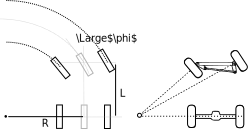
\includegraphics[width=0.9\textwidth]{figs/ackermann.png}
    \def\svgwidth{0.9\textwidth}
    \import{./figs/}{ackermann.pdf_tex}
    \caption{Left: Kinematics of car-like steering and the equivalent bicycle model. Right: Mechanism of an Ackermann vehicle.}
    \label{fig:ackermann}
\end{figure}

Let the car have the shape of a box with length $L$ between rear and front axis. Let the center point of the common circle described by all wheels be distance $ R$ from the car's longitudinal center line.  Then, the steering angle $ \phi$ is given by

\begin{equation}\label{eq:ackermann}
\tan \phi = \frac{L}{R}
\end{equation}

The angles of the left and the right wheel, $ \phi_l$ and $ \phi_r$ can be calculated using the fact that all wheels of the car rotate around circles with a common center point. With the distance between the two front wheels $l$, we can write:
\begin{eqnarray}
\frac{L}{R-l/2}&=\tan{(\phi_r)} \nonumber \\
\frac{L}{R+l/2}&=\tan{(\phi_l)}
\end{eqnarray}
This is important, as it allows us to calculate the resulting wheel angles resulting from a specific angle $\phi$ and test whether they are within the constraints of the actual vehicle.

Assuming the wheel speed to be $\dot{\omega}$ and the wheel radius $r$, we can calculate the speeds in the robot's coordinate frame as:
\begin{eqnarray}
\dot{x}_r&=\dot{\omega}r \nonumber \\
\dot{y}_r&=0\\
\dot{\theta}_r&=\frac{\dot{\omega}r\tan\phi}{L} \nonumber
\end{eqnarray}
using (\ref{eq:ackermann}) to calculate the circle radius $R$.

\subsection{The Denavit-Hartenberg notation}\label{sec:kinematics:dh}

So far, we have considered the forward kinematics of wheeled mechanisms and simple arms and derived relationships between actuator parameters and velocities using basic trigonometry.
In the case of multi-link arms (which is the vast majority of robot manipulators in existence), the approach detailed in \cref{sec:kinematics:fwkarm} is difficult to scale, and alternative solutions are needed.
Interestingly, we can think of the forward kinematics as a chain of homogeneous transformations with respect to a coordinate system mounted at the base of a manipulator or a fixed position in the room.
Deriving these transformations can be confusing and can be facilitated by following a ``recipe'' such as the one conceived by Denavit and Hartenberg in $1955$ \td{citation?}.
The so-called Denavit-Hartenberg (DH)\index{Denavit-Hartenberg parameters} representation has evolved as a \textsl{de-facto} standard and can easily be automatized, i.e., applied to a 3D model of a robotic arm, e.g. \td{Nikolaus, what do you meant here?}

A manipulator consists of a series of typically rigid links that are connected by joints.
In the vast majority of cases, a joint can either be revolute (i.e. change its angle/orientation) or prismatic (i.e. change its length).
Knowing the robot's kinematic properties (e.g. the length of all rigid links, similarly to $l_1$ and $l_2$ in \cref{fig:fwk2dofarm}), the pose of its end-effector is fully described by its joint configuration (angle for revolute joints, length for prismatic joints).

%In industrial manipulators, the number of joints is usually equal to the degrees of freedom of the manipulator. As most manipulators are holonomic, the forward kinematics allow you---unlike on non-holonomic wheeled platforms---to directly relate absolute positions of joints with absolute positions in Cartesian space. It is also possible to derive equations that relate the speed of the joints to speed in Cartesian space. Like for wheeled platforms, this can be achieved via a Jacobian matrix.  At certain positions, the mapping provided by the Jacobian is not invertible, i.e., some velocities in Cartesian space are unachievable. These points are called singularities.

\screencast{http://youtu.be/rA9tm0gTln8}{denavithartenberg}

\begin{figure}[!t]
    \centering
    % 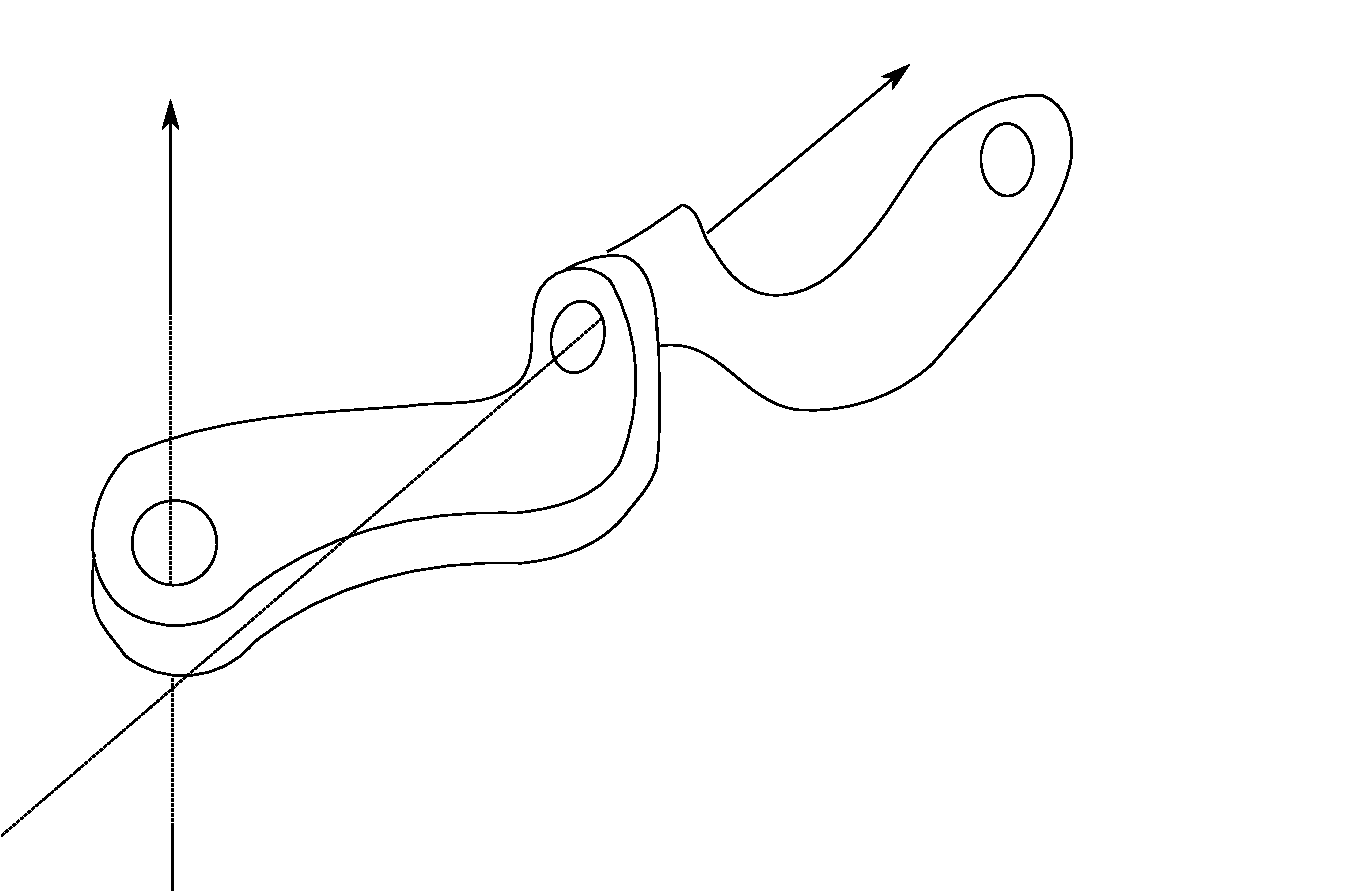
\includegraphics[width=\textwidth]{figs/denavit-hartenberg.png}
    \def\svgwidth{\textwidth}
    \import{./figs/}{denavit-hartenberg.pdf_tex}
    \caption{Example of selected Denavit-Hartenberg parameters for three sequential revolute joints. The z-axes of joint $i$ and $i+1$ are parallel.}
    \label{fig:denavit}
\end{figure}

In order to use the DH-convention, we first need to define a coordinate system at each joint. With reference to \cref{fig:denavit}, we choose the $z-$axis to be the axis of rotation for a revolute joint and the axis of translation for a prismatic joint.
We can now find the common normal between the $z-$axes of two subsequent joints, i.e. a line that is orthogonal to each $z-$axis and intersects both.
With the direction of the $x-$axis at the base arbitrary, subsequent $x-$axes are chosen such that they lie on the common normal shared between two joints.
Whereas the direction of the $z-$axis is given by the positive direction of rotation (right-hand rule), the $x-$axis points away from the previous joint.
This allows defining the $y-$axis using the right-hand rule.
Note that these rules, in particular the requirement that $x$-axes lie along the commom normal, might result in coordinate systems with their origins outside the joint: this is not relevant as the kinematics of a manipulator is a mathematical representation that needs to represent the geometric and kinematic properties of the robot, and does not need to bear any physical correspondence.
%
The transformation between two joints is then fully described by the following four parameters:
\begin{enumerate}
\item The length $r$ (sometimes, $a$ is used) of the common normal between the $z$-axes of two joints $i$ and $i-1$ (link length).
\item The angle $ \alpha$ between the z-axes of the two joints with respect to the common normal (link twist), i.e. the angle between the old and the new $z$-axis, measured about the common normal.
\item The distance $d$ between the joint axes (link offset), i.e. the offset along the previous $z$-axis to the common normal.
\item The rotation $ \theta$ around the common axis along which the link offset is measured (joint angle), i.e. the angle from the old $x$-axis to the new $x$-axis, about the previous $z$-axis.
\end{enumerate}

Two of the above D-H parameters describe the link between the joints, and the other two describe the link's connection to a neighboring link.
Depending on the link/joint type, these numbers are fixed by the specific mechanical instance of the robot or can be controlled.
For example, in a revolute joint $ \theta$ is the varying joint angle, while all other quantities are fixed.  Similarly, for a prismatic joint $d$ is the joint variable. An example of two revolute joints is shown in \cref{fig:denavit}.

The final coordinate transform from one link ($i-1$) to another ($i$) can now be constructed by concatenating the four steps above, which are nothing but a series of rotations and translations, one for each DH parameter:
%
\begin{equation}\label{eq:kinematics:dh:composition}
_{n-1}^nT=T_z'(d_n) R_z'(\theta_n) T_x(r_n)  R_x(\alpha_n)
\end{equation}
with
\begin{equation}
T_z'(d_n)=
\left[
\begin{array}{ccc|c}
1 & 0 & 0 & 0\\
0 & 1 & 0 & 0\\
0 & 0 & 1 & d_n\\
\hline
0 & 0 & 0 & 1
\end{array}
\right]
\enskip
R_z'(\theta_n)=\left[
\begin{array}{ccc|c}
\cos\theta_n & -\sin\theta_n & 0 & 0\\
\sin\theta_n & \cos\theta_n & 0 & 0\\
0 & 0 & 1 & 0\\
\hline
0 & 0 & 0 & 1
\end{array}
\right]
\end{equation}
and
\begin{equation}
T_x(r_n)=
\left[
\begin{array}{ccc|c}
1 & 0 & 0 & r_n\\
0 & 1 & 0 & 0\\
0 & 0 & 1 & 0\\
\hline
0 & 0 & 0 & 1
\end{array}
\right]
\enskip
R_x(\alpha_n)=\left[
\begin{array}{ccc|c}
1 & 0 & 0 & 0\\
0 & \cos\alpha_n & -\sin\alpha_n & 0\\
0 & \sin\alpha_n & \cos\alpha_n & 0\\
\hline
0 & 0 & 0 & 1
\end{array}
\right]
\end{equation}
%
These are a translation of $d_n$ along the previous z-axis ($T_z'(d_n)$), a rotation of $\theta_n$ about the previous z-axis ($R_z'(\theta_n)$), a translation of $r_n$ along the new $x$-axis ($T_x(r_n)$)and a rotation of $\alpha_n$ around the new $x$-axis ($R_x(\alpha_n)$).
%
By replacing each element in \cref{eq:kinematics:dh:composition}, the following matrix is created:
\begin{eqnarray}
_{n-1}^nT&=
\left[
\begin{array}{ccc|c}
\cos \theta_n & -\sin \theta_n \cos\alpha_n & \sin\theta_n \sin\alpha_n & r_n \cos\theta_n\\
\sin \theta_n & \cos\theta_n \cos\alpha_n & -\cos\theta_n\sin\alpha_n & r_n \sin\theta_n\\
0 & \sin\alpha_n & \cos\alpha_n & d_n \nonumber \\
\hline
0 & 0 & 0 & 1
\end{array}
\right]\\
&=
\left[
\begin{array}{c|c}
R & t\\
\hline
0 \quad 0 \quad 0 & 1
\end{array}
\right]
\end{eqnarray}
where $R$ is the $3\times3$ rotation matrix and $t$ is the $3\times1$ translation vector.

Like for any homogeneous transform, the inverse $_{n-1}^nT^{-1}n$ is given by
\begin{equation}
^{n-1}_nT=\left[
\begin{array}{c|c}
R^{-1} & -R^{-1}T\\
\hline
0 \quad 0 \quad 0 \quad 1
\end{array}
\right]
\end{equation}
with the inverse of $R$ simply being its transpose, $R^{-1}=R^T$.

Similar to the concatenation of transformations detailed in \cref{sec:kinematics:coordsystems:concatenation}, $_{n-1}^nT$ in \cref{eq:kinematics:dh:composition} can be concatenated with the other transformation matrices relative to the remaining links in order to compute a the full kinematics of the robot arm from the base reference frame up to the end-effector.

%!TEX root = ../book.tex
\section{Inverse Kinematics}\label{sec:kinematics:ik}

The forward kinematics of a system are computed by means of a transformation matrix from the base of a manipulator (or fixed location, such as the corner of a room) to the end-effector of a manipulator (or a mobile robot).
As such, they are an exact description of the pose of the robot and they fully characterize its kinematic state.
Inverse Kinematics deal with the opposite problem: finding a joint configuration that results in a desired pose at the end effector.
To achieve this goal, we will need to solve the forward kinematics equations for joint angles as a function of the desired pose.
With reference to \cref{eq:kinematics:forward}, inverse kinematics aims to solve the following:
\begin{equation}\label{eq:kinematics:inverse}
q = f^{-1} (r)\ , \qquad f^{-1} : \mathbb{R}^m \rightarrow \mathbb{R}^n \ ,
\end{equation}
with a notation similar to \cref{eq:kinematics:forward}.
For a mobile robot, we can do this only for velocities in the local coordinate system, and need more sophisticated methods to calculate appropriate trajectories. We will discuss this in depth in \cref{sec:kinematics:diff}.

\subsection{Solvability}

\cref{eq:kinematics:inverse} is the inverted version of \cref{eq:kinematics:forward}, and is heavily non-linear except for trivial mechanisms.
Therefore, it makes sense to briefly think about whether we can solve it at all for specific parameters before trying.
Here, the workspace of a robot becomes important. The workspace is the sub-space that can be reached by the robot in any configuration.
Clearly, there will be no solutions for the inverse kinematic problem outside of the workspace of the robot.

A second question to ask is how many solutions we actually expect to exist and what it means to have multiple solutions \textsl{geometrically}.
Multiple solutions to achieve a desired pose correspond to multiple ways in which a robot can reach a target (i.e., joint configurations).
For example a three-link arm that wants to reach a point that can be reached without fully extending all links (which would have only a single solution) can do this by either folding its links in a concave or a convex fashion.
Reasoning about how many solutions will exist for a given mechanism and desired pose quickly becomes non-intuitive.
For example, a 6-DOF arm can reach certain points with up to $16$ different configurations!

\subsection{Inverse Kinematics of a Simple Manipulator Arm}\label{sec:kinematics:inverse:arm}

We will now look at the inverse kinematics of the $2-$link arm that we introduced in \cref{fig:fwk2dofarm}. We need to solve the equations determining the robot's forward kinematics by solving for $\alpha$ and $ \beta$.
This is tricky, however, as we have to deal with more complicated trigonometric expressions than the forward kinematics case.

To build an intuition, assume there to be only one link, $l_1$.  Solving (\ref{eq:cosxl1}) for $\alpha$ yields to two distinct solutions:

\begin{equation}
\alpha = \pm \cos^{-1}\frac{x_1}{l_1},
\end{equation}
as cosine is symmetric for positive and negative values.
Indeed, for any possible position on the $x-$axis ranging from $-l_1$ to $l_1$, there exist two solutions: the first one with the arm above the table, and the other one with the arm below it.
At the extremes of the workspace, both solutions are the same.

%\begin{verbatim}
%sol = Solve[Sin[a + b] + Sin[a] == y
%             && Cos[a + b] + Cos[a] == x,
%            {a, b}];
%min = sol /. {x -> 1, y -> 1}
%\end{verbatim}

Solving \ref{eq:fwk2dofarm} for $\alpha$ and $\beta$ adds two additional solutions that are cumbersome to reproduce here, involving terms of $x$ and $y$ to the sixth power, and is left as an exercise to the reader, for example using an online symbolic solver.


What will drastically simplify this problem, is to not only specify the desired position, but also the orientation $\theta$ of the end-effector. In this case, a desired pose can be specified in the following form
\begin{equation}
\left[
\begin{array}{cccc}
cos\theta & -sin\theta & 0 & x\\
sin\theta & cos\theta & 0 & y\\
0 & 0 & 1 & 0\\
0 & 0 & 0 & 1
\end{array}
\right].
\end{equation}
A solution can now be found by simply equating the individual entries of the transformation (\ref{eq:2armtrans}) with those of the desired pose. Specifically, we can observe:
\begin{eqnarray}
cos\theta &=& cos(\alpha+\beta)\\
\nonumber
x &=& c_{\alpha\beta}l_2+c_\alpha l_1\\
\nonumber
y &=& s_{\alpha\beta}l_2+s_\alpha l_1
\end{eqnarray}
These can be reduced to
\begin{eqnarray}
\theta &=& \alpha + \beta \nonumber \\
c_\alpha &=& \frac{c_{\alpha\beta}l_2-x}{l_1}=\frac{c_\theta l_2-x}{l_1} \\
s_\alpha &=& \frac{s_{\alpha\beta}l_2-y}{l_1}=\frac{s_\theta l_2-y}{l_1} \nonumber
\end{eqnarray}
Providing the orientation of the robot in addition to the desired position therefore allows solving for $\alpha$ and $\beta$ just as a function of $x$, $y$ and $\theta$.

The main issue with the geometric approach detailed above is that it does not scale easily with an increase of DoF at the joints, and it quickly becomes unwieldy with more dimensions.
For higher-DoF platforms, we can calculate a \textsl{numerical solution} using an approach that we will later see is very similar to path planning in mobile robotics.
To this end, we will take an optimization-based approach: first we calculate a measure of error between the current solution and the desired one, and then change the joint configuration in a way that minimizes this error.
In our example, the measure of error is the Euclidean distance between the current end-effector pose (given by the forward kinematics equations in \cref{eq:fwk2dofarm}) and the desired solution $[x,y]$ in configuration space, i.e. (assuming $l_1=l_2=1$ for simplicity):
% To do this, you need to solve the forward kinematics for every point in configuration space and use the Euclidean distance to the desired target as height.
\begin{equation}\label{eq:kinematics:inverse:numerical}
f_{x,y}(\alpha,\beta)=\sqrt{\left(s_{\alpha\beta} + s_\alpha - y\right)^2 + \left(c_{\alpha\beta}+c_\alpha - x\right)^2}
\end{equation}
Here, the first two terms in parentheses are given by the forward kinematics of the robot, whereas the third term in the parentheses is the desired $y$ and $x$ position, respectively.
\cref{eq:kinematics:inverse:numerical} can be plotted as a 3D function of $\alpha$ and $\beta$, our joint-space variables.
% This is plotted for $\alpha=[-\pi/2,\pi/2]$ and $\beta=[-\pi,\pi]$ and $x=1$, $y=1$ in Figure~\ref{fig:inversekinematics}.
As shown in \cref{fig:inversekinematics} this function has a minima, in this case zero, for values of $\alpha$ and $\beta$ that bring the manipulator to $(1,1)$. These values are $(\alpha \rightarrow 0, b \rightarrow -\frac{\pi}{2})$ and $(\alpha \rightarrow -\frac{\pi}{2}, b \rightarrow \frac{\pi}{2})$.

\begin{figure}
    \centering
        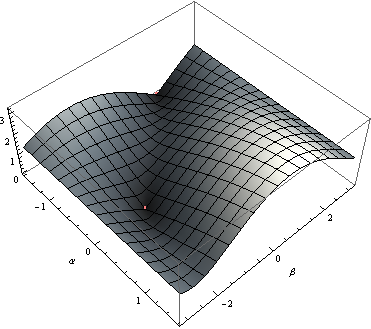
\includegraphics[width=0.8\textwidth]{figs/kinematics/inversekinematics}
    \caption{Distance to $(x=1,y=1)$ over the configuration space of a two-arm manipulator. Minima corresponds to exact inverse kinematic solutions.}
    \label{fig:inversekinematics}
\end{figure}

You can now think about inverse kinematics as a path finding problem from anywhere in the configuration space to the nearest minima. A more formalized approach to this will be discussed in \cref{sec:kinematics:inverse:feedbackcontrol}. How to find the shortest path in space, that is finding the shortest route for a robot to get from A to B, is one of the subjects covered within \cref{chap:pathplanning}.



%!TEX root = ../book.tex
\section{Differential Kinematics}\label{sec:kinematics:diff}

The two-link arm in Figure~\ref{fig:fwk2dofarm} involved only two free parameters, but was already pretty complex to solve analytically if the end-effector pose was not specified.
One can imagine that things become very hard with more degrees of freedom or more complex geometries (mechanisms in which some axes intersect are simpler to solve than others, for example).
It is worth noting that, so far, we have analyzed the geometry of motion of a robot at its simplest level of abstraction, i.e. in the space of positions. This abstraction becomes useless as soon as the order of motions matters. For example, in a differential wheel robot, turning the left wheel first and then the right wheel will lead to a very different position then turning the right wheel first and then the left wheel. This is not the case in a robotic arm with two links, which will arrive at the same position no matter which joint will be moved first. 

In order to include a notion of temporal evolution of the robot configuration, it is convenient to shift toward a slightly more complex abstraction, that is the space of generalized velocities. This modeling is called \textsl{differential kinematics}\index{Differential Kinematics}, as velocities are the time derivative (i.e. the differential) of positions.
Similarly to before, with ``generalized velocities'' we mean ``any velocity-equivalent quantity needed to describe the element'', as we will detail below.

\subsection{Forward Differential Kinematics}\label{sec:kinematics:diff:fwd}

Forward differential kinematics deals with the problem of computing an expression that relates the generalized velocities at the joints (i.e. the ``speed'' of our motors) to the generalized velocity of the robot's end-effector. In all, it is the corresponding differential version of \cref{eq:kinematics:forward}.
% This is known as \textsl{Differential Kinematics}\index{Differential Kinematics}, as we are operating in the space of velocities, which are the derivative of positions.
Let the translational speed of a robot be given by:
\begin{equation}
v=\left[\begin{array}{c}
\dot{x}\\
\dot{y}\\
\dot{z}
\end{array}
\right].
\end{equation}
As the robot can potentially not only translate, but also rotate, we also need to specify its angular velocity. Let these velocities be given as a vector $\omega$:
\begin{equation}
\omega=\left[\begin{array}{c}
\omega_x\\
\omega_y\\
\omega_z
\end{array}
\right].
\end{equation}
We can now write translational and rotational velocities in a $6\times1$ generalized velocity vector as $\nu = [v \ \omega]^T$.
This notation is also called a \textsl{velocity twist}.\index{Twist (velocity)}\index{Velocity Twist} %By convention, the speed of rotation is given by the magnitude (or length) of this vector.
Let the generalized configuration in joint space (i.e. joint angles/positions) be $q=[q_1, \ldots, q_n]^T$; therefore, we can define the set of joint speeds as $\dot{q}=[\dot{q}_1, \ldots, \dot{q}_n]^T$.
%
We now want to compute the differential kinematics version of \cref{eq:kinematics:forward}, and in this case relate joint velocities $\dot{q}$ with end-effector velocities $[v \ \omega]^T$. A simple derivation of \cref{eq:kinematics:forward} with respect to time gives:
\begin{equation}\label{eq:kinematics:diff:fwd:short}
\nu = [v \quad \omega]^T=J(q)\cdot [\dot{q}_1,\ldots,\dot{q}_n]^T = J(q) \cdot \dot{q} \ ,
\end{equation}
which is our forward differential kinematics equation. $J(q)$ is known as the \textsl{Jacobian matrix}\index{Jacobian Matrix}; it is function of the joint configuration $q$, and contains all the partial derivatives of $f$ that relate every joint angle to every velocity. In practice, $J$ looks like the following:

\begin{equation}\label{eq:kinematics:diff:fwd}
\nu = \left[\begin{array}{c}v\\\omega\end{array}\right]=
\left[\begin{array}{c}\dot{x}\\
\dot{y}\\
\dot{z}\\
\omega_x\\
\omega_y\\
\omega_z\end{array}\right]=
\left[\begin{array}{cccc}\frac{\partial{x}}{\partial{q_1}} & \frac{\partial{x}}{\partial{q_2}} & \ldots & \frac{\partial{x}}{\partial{q_n}}\\\frac{\partial{y}}{\partial{q_1}} & \frac{\partial{y}}{\partial{q_2}} & \ldots & \frac{\partial{y}}{\partial{q_n}}\\\vdots & \vdots & \vdots & \vdots\\\frac{\partial{\omega_z}}{\partial{q_1}} & \frac{\partial{\omega_z}}{\partial{q_2}} & \ldots & \frac{\partial{\omega_z}}{\partial{q_n}}\end{array}\right]\left[\begin{array}{c}\dot{q}_1\\\vdots\\\dot{q}_n\end{array}\right] = J (q) \cdot \dot{q}
\end{equation}

This notation is important as it tells us how small changes in joint space will affect the end-effector's position in Cartesian space. Better yet, the forward kinematics of a mechanism and its analytical derivative can always be calculated, which allows us to calculate numerical values for the entries of matrix $J$ for every possible joint angle/position.

\subsection{Forward Kinematics of a Differential Wheels Robot}\label{sec:kinematics:fwk:mobile}

After abstractly considering differential kinematics in the previous section, we will now study a mechanism for which general non-differential kinematic models do not exist. We recall that the pose of a robotic manipulator is uniquely defined by its joint angles, which can be estimated using encoders.
However, this is not the case for a mobile robot.
Here, the encoder values simply refer to wheel orientation and need to be integrated over time in order to assess the robot's position with respect to the world's frame of reference; as we will later see, this is a great source of uncertainty.
What complicates matters is that for so-called \textsl{non-holonomic} systems, it is not sufficient to simply measure the distance that each wheel traveled, but also when each movement was executed.

\begin{figure}[!t]
    \small
    \centering
    % 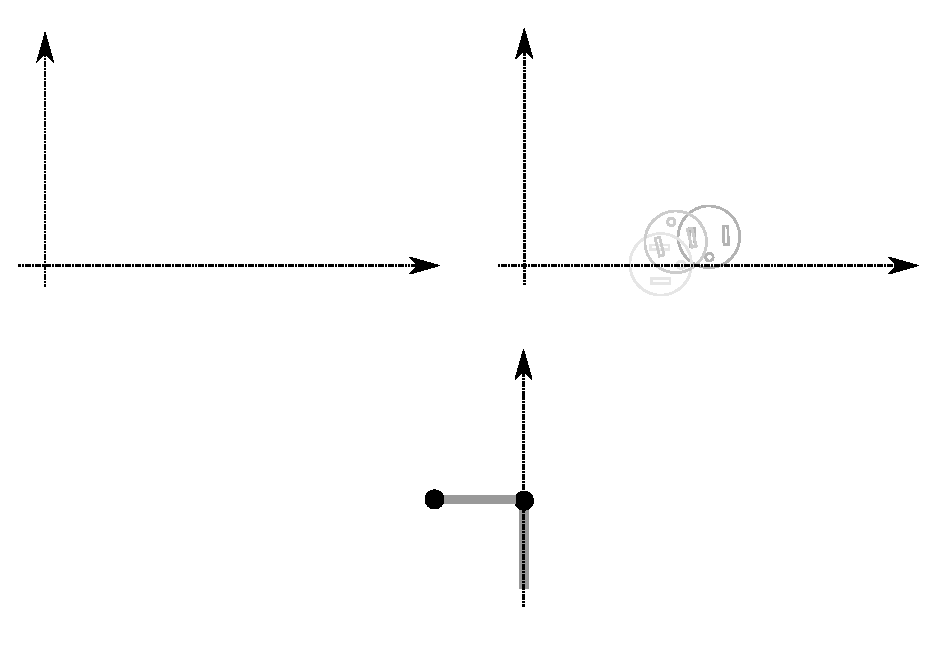
\includegraphics[width=0.95\textwidth]{figs/holonomy.png}
    \def\svgwidth{\textwidth}
    \import{./figs/kinematics/}{holonomy.pdf_tex}
    \caption{Configuration or joint space (left) and workspace or operational space (right) for a non-holonomic mobile robot (top) and a holonomic manipulator (bottom). Closed trajectories in configuration space result in closed trajectories in the workspace if the robot's kinematics is holonomic.}
    \label{fig:holonomy}
\end{figure}

A system is non-holonomic\index{Non-holonomic}\index{Holonomic} when closed trajectories in its configuration space may not have it return to its original state.
 % (reminder: the configuration or joint space space of a two-link robotic arm is spanned by the possible values of each angle).
A robot arm is holonomic because each joint position corresponds to a unique position in space (\cref{fig:holonomy}, bottom):
a generic joint-space trajectory that comes back to the starting point will position the robot's end-effector at the exact same position in operational space.
A train on a track is holonomic too: moving its wheels backwards by the same amount they have been moving forward brings the train to the exact same position in space.
Conversely, a car and a differential-wheel robot are non-holonomic vehicles (\cref{fig:holonomy}, top): performing a straight line and then a right-turn leads to the same amount of wheel rotation than doing a right turn first and then going in a straight line; however, getting the robot to its initial position requires not only to rewind both wheels by the same amount, but also getting their relative speeds right.
The configuration and corresponding workspace trajectories for a non-holonomic and a holonomic robot are shown in \cref{fig:holonomy}.
Here, a robot first moves on a straight line, i.e. both wheels turn an equal amount.
Then, the left wheel remains fixed and only the right wheel turns forward.
Then, the right wheel remain fixed and the left wheel turns backward.
Finally, the right wheel turns backward, arriving at the initial encoder values (zero).
Yet, the robot does not return to its origin. Performing a similar trajectory in the configuration space of a two-link manipulator instead, lets the robot return to its initial position.

It should be clear by now that for a mobile robot, not only traveled distance per wheel matters, but also the \textsl{speed} of each wheel as a function of time.
Interestingly, this information was not required to uniquely determine the pose of a manipulating arm.
Let's introduce the following conventions.
We will establish a world coordinate system $\{I\}$---which is known as the inertial frame by convention (see \cref{fig:mobilerobot}).
We establish a coordinate system $\{R\}$ on the robot and express the robot's speed $^R\dot{\xi}$ as a vector $ ^R\dot{\xi}=[^R\dot{x}, ^R\dot{y}, ^R\dot{\theta}]^T$. Here $^R\dot{x}$ and $^R\dot{y}$ correspond to the speed along the $x$ and $y$ directions in $\{R\}$, whereas $^R\dot{\theta}$ corresponds to the rotation velocity around the $z-$axis, that you can imagine to be sticking out of the ground.
We denote speeds with dots over the variable name, as speed is simply the derivative of distance.
Now, let's think about the robot's position in $\{R\}$. It is always zero, as the coordinate system is fixed on the robot itself.
Therefore, velocities are the only interesting quantities in this coordinate system and we need to understand how velocities in $\{R\}$ map to positions in $\{I\}$, which we denote by $^I\xi=[^Ix, ^Iy, ^I\theta]^T$. These coordinate systems are shown in \cref{fig:mobilerobot}.

\begin{figure}[htb!]
    \centering
    % 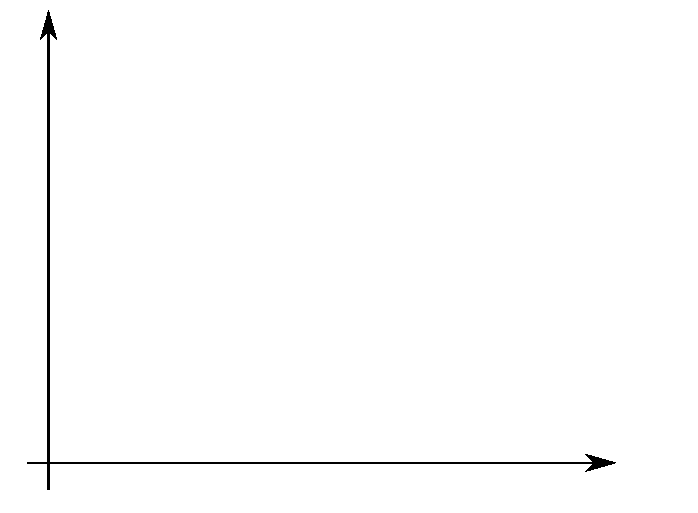
\includegraphics[width=0.85\textwidth]{figs/mobilerobot.png}
    \def\svgwidth{0.85\textwidth}
    \import{./figs/kinematics/}{mobilerobot.pdf_tex}
    \caption{Mobile robot with local coordinate system \{R\} and world frame \{I\}. The arrows indicate the positive direction of position and orientation vectors.}
    \label{fig:mobilerobot}
\end{figure}

Notice that the positioning of the coordinate frames and their orientation are arbitrary. Here, we choose to place the coordinate system in the center of the robot's axle and align $^Rx$ with its default driving direction.
In order to calculate the robot's position in the inertial frame, we need to first find out how speed in the robot coordinate frame maps to speed in the inertial frame.
This can be done again by employing trigonometry. There is only one complication: a movement into the robot's $x-$axis might lead to movement along both the $x-$axis and the $y-$axis of the world coordinate frame ${I}$. By looking at \cref{fig:mobilerobot}, we can derive the following components to $\dot{x}_I$. First,
\begin{equation}
\dot{x}_{I,x}=cos(\theta) \dot{x}_R.
\end{equation}

There is also a component of motion coming from $ \dot{y}_R$ (ignoring the kinematic constraints for now, see below).  For negative $ \theta$, as in \cref{fig:mobilerobot}, a move along $y_R$ would let the robot move into positive $ X_I$ direction. The projection from $ \dot{y}_R$ is therefore given by
\begin{equation}
\dot{x_{I,y}}=-sin(\theta)\dot{y_R}.
\end{equation}
We can now write
\begin{equation}
\dot{x_I}=cos(\theta) \dot{x_R} - sin(\theta) \dot{y_R}.
\end{equation}
Similar reasoning leads to:
\begin{equation}
\dot{y_I}=sin(\theta) \dot{x_R} + cos(\theta) \dot{y_R}
\end{equation}
and
\begin{equation}
\dot{\theta_I}=\dot{\theta_R}
\end{equation}
which is the case because both robot's and world coordinate system share the same z-axis in this example. We can now conveniently write
\begin{equation}
\dot{\xi_I}=^I_RT(\theta)\dot{\xi_R}
\end{equation}
with
\begin{equation}
^I_RT(\theta)=\left[\begin{array}{ccc}
cos(\theta) & -sin(\theta) & 0 \\
sin(\theta) & cos(\theta) & 0 \\
0 & 0 & 1\end{array}\right]
\end{equation}

We are now left with the problem of how to calculate the speed $ \dot{\xi_R}$ in robot coordinates. For this, we make use of the \textsl{kinematic constraints}\index{Kinematic constraints} of the robotic wheels.
For a standard wheel in an ideal case scenario, the kinematic constraints are that every rotation of the wheel leads to strictly forward or backward motion and does not allow side-way motion or sliding. We can therefore calculate the forward speed of a wheel $ \dot{x}$ using its rotational speed $ \dot{\phi}$ (assuming the encoder value/angle is expressed as $ \phi$) and radius $ r$ by
\begin{equation}
\dot{x}=\dot{\phi}r.
\end{equation}
This becomes apparent when considering that the circumference of a wheel with radius $r$ is $2\pi r$. The distance a wheel rolls when turned by the angle $ \phi$ (in radians) is therefore $ x=\phi r$, see also \cref{fig:wheelrotation}, right. Taking the derivative of this expression on both sides leads to the above expression.

\begin{figure}[htb!]
    \centering
    % 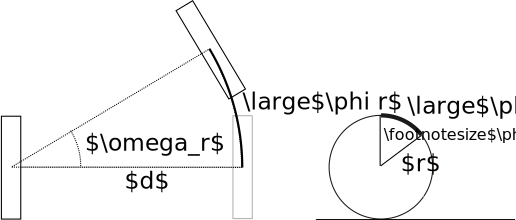
\includegraphics[width=0.9\textwidth]{figs/wheelrotation.png}
    \def\svgwidth{\textwidth}
    \import{./figs/kinematics/}{wheelrotation_2.pdf_tex}
    \caption{Left: Differential wheel robot pivoting around its left wheel first and its right wheel next. For infinitesimal motion, it is possible to decouple left and right wheel to simplify computation of the forward kinematics. Right: A wheel with radius $r$ moves by $\phi r$ when rotated by $\phi$ degrees.}
    \label{fig:wheelrotation}
\end{figure}

How each of the two wheels in our example contributes to the speed of the robot's center---where its coordinate system is anchored---requires the following trick: we calculate the contribution of each individual wheel while assuming all other wheels remaining un-actuated (see \cref{fig:wheelrotation}, left).
In this example, the left wheel will move of $r \phi_l$, and the right wheel will move of $r \phi_r$, which in the space of velocities will become $r\dot{\phi_l}$ and $r\dot{\phi_r}$ respectively.
Then, the distance traveled by the center point is exactly half of that traveled by each individual wheel, assuming the non-actuated wheel rotating around its ground contact point (\cref{fig:wheelrotation}). We can therefore write:
\begin{equation}
\dot{x_R}=\frac{1}{2}\left( r\dot{\phi_l} + r\dot{\phi_r} \right)=\frac{r\dot{\phi_l}}{2}+\frac{r\dot{\phi_r}}{2}
\end{equation}
given the speeds $ \dot{\phi_l}$ and $ \dot{\phi_r}$ of the left and the right wheel, respectively.

\begin{mdframed}
Think about how the robot's speed along its y-axis is affected by the wheel speed given the coordinate system in the drawing above. Think about the kinematic constraints that the standard wheels impose.
\end{mdframed}

Hard to believe at first, but the speed of the robot along its y-axis is always zero. This is because the constraints of the standard wheel tell us that the robot can never slide.
We are now left with calculating the rotation of the robot around its z-axis. This rotation can be seen when imaging the robot's wheels spinning in opposite directions. Then the robot does not move forward, but spins in place.
We will again consider each wheel independently. Assuming the left wheel to be non-actuated, spinning the right wheel forwards will lead to counter-clockwise rotation. Given an axle diameter (distance between the robot's wheels) $d$, we can now write
\begin{equation}
\omega_r d = \phi_r r
\end{equation}
with $\omega_r$ the angle of rotation around the left wheel (\cref{fig:wheelrotation}, left). Taking the derivative on both sides yields speeds and we can write
\begin{equation}
\dot{\omega_r} = \frac{\dot{\phi_r} r}{d}
\end{equation}
Adding the rotation speeds up (with the one around the right wheel being negative based on the right-hand grip rule), leads to:
%
\begin{equation}
\dot{\theta}=\frac{\dot{\phi_r} r}{d}-\frac{\dot{\phi_l} r}{d}
\end{equation}
%
Putting it all together, we can finally write:

\begin{equation}\label{eq:kinematics:forward:mobile}
\left[\begin{array}{c} \dot{x_I}\\\dot{y_I}\\\dot{\theta}\end{array}\right]=\left[\begin{array}{ccc}
cos(\theta) & -sin(\theta) & 0 \\
sin(\theta) & cos(\theta) & 0 \\
0 & 0 & 1\end{array}\right]\left[\begin{array}{c}\frac{r\dot{\phi_l}}{2}+\frac{r\dot{\phi_r}}{2}\\0\\\frac{\dot{\phi_r} r}{d}-\frac{\dot{\phi_l} r}{d}\end{array}\right]
\end{equation}

The interested reader might want to compare this form with \cref{eq:kinematics:diff:fwd}, the general Jacobian form of differential kinematics. For this, we ignore the rotation matrix in \cref{eq:kinematics:forward:mobile} and rewrite its second term in matrix notation:

\begin{equation}
\left[\begin{array}{c} \dot{x_R}\\\dot{y_R}\\\dot{\theta}\end{array}\right]=\left[\begin{array}{cc}
\frac{r}{2} & \frac{r}{2}\\
0 & 0 \\
\frac{r}{d} & -\frac{r}{d} \end{array}\right]
\left[\begin{array}{c}\dot{\phi_l}\\\dot{\phi_r}\end{array}\right]
=
\left[\begin{array}{cc}
\frac{\partial{x_R}}{\partial{\dot{\phi}_l}} & \frac{\partial{x_R}}{\partial{\dot{\phi}_r}}\\\frac{\partial{y_R}}{\partial{\dot{\phi}_l}} & \frac{\partial{y_R}}{\partial{\dot{\phi}_r}}\\\frac{\partial{\theta}}{\partial{\dot{\phi}_l}} & \frac{\partial{\theta}}{\partial{\dot{\phi}_l}} \end{array}\right]
\left[\begin{array}{c}
\dot{\phi_l}\\\dot{\phi_r}
\end{array}\right]
\end{equation}
With $X_R=\left(\frac{r\dot{\phi}_l}{2}+\frac{r\dot{\phi}_r}{2})\right)t$ and similar expressions for $\theta$, we observe the validity of the Jacobian approach. 



\subsubsection{From Forward Kinematics to Odometry}

\cref{eq:kinematics:forward:mobile} only provides us with the relationship between the robot's wheel speed and its speed in the inertial frame.
Calculating its actual pose in the inertial frame is known as \textsl{odometry}\index{Odometry}. Technically, it requires integrating \cref{eq:kinematics:forward:mobile} from 0 to the current time $T$.
As this is not possible but for very special cases, one can approximate the robot's pose by summing up speeds over discrete time intervals, or more precisely:
\begin{equation}
\left[\begin{array}{c} {x_I}(T)\\{y_I}(T)\\{\theta}(T)\end{array}\right]=
\int_0^T \left[\begin{array}{c} \dot{x_I}(t)\\\dot{y_I}(t)\\\dot{\theta}(t)\end{array}\right] dt \approx
\sum_{k=0}^{k=T}\left[\begin{array}{c} \Delta{x_I}(k)\\\Delta{y_I}(k)\\\Delta{\theta}(k)\end{array}\right]\Delta t
\end{equation} which can be calculated incrementally as
\begin{equation}\label{eq:odometry}
x_I(k+1)=x_I(k)+\Delta x (k) \Delta t
\end{equation}
using $\Delta x(k) \approx \dot{x_I}(t)$ and similar expressions for $y_I$ and $\theta$. Note that \cref{eq:odometry} is just an approximation. The larger $\Delta t$ becomes, the more inaccurate this approximation becomes as the robot's speed might change during the interval.

\begin{mdframed}
\noindent Don't let the notion of an integral worry you! As robots' computers are fundamentally discrete, integrals usually turn into sums, which are nothing than for-loops.
\end{mdframed}

\subsection{Forward kinematics of Car-like steering}\label{sec:kinematics:fwk:car}

Differential wheel drives are very popular in mobile robotics as they are very easy to build, maintain, and control.
Although not holonomic, a differential drive can approximate the function of a fully holonomic robot by first driving on the spot to achieve the desired heading and then driving straight.
Drawbacks of the differential drive are its reliance on a caster wheel, which performs poorly at high speeds, and difficulties in driving straight lines as this requires both motors to drive at the exact same speed.

These drawbacks are mitigated by car-like mechanisms, which are driven by a single motor and can steer their front wheels. This mechanism is known as ``Ackermann steering''. \index{Ackermann steering}
Ackermann steering should not be confused with ``turntable'' steering \index{Turntable steering} where the front wheels are fixed on an axis with central pivot point.
Instead, each wheel has its own pivot point and the system is constrained in such a way that all wheels of the car drive on circles with a common center point, avoiding skid.
As the Ackermann mechanism lets all wheels drive on circles with a common center point, its kinematics can be approximated by those of a tricycle with rear-wheel drive, or even simpler by a bicycle. This is shown in \cref{fig:ackermann}.

\begin{figure}[htb!]
    \centering
    % 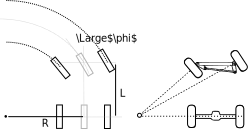
\includegraphics[width=0.9\textwidth]{figs/ackermann.png}
    \def\svgwidth{0.9\textwidth}
    \import{./figs/kinematics/}{ackermann.pdf_tex}
    \caption{Left: Kinematics of car-like steering and the equivalent bicycle model. Right: Mechanism of an Ackermann vehicle.}
    \label{fig:ackermann}
\end{figure}

Let the car have the shape of a box with length $L$ between rear and front axis. Let the center point of the common circle described by all wheels be distance $ R$ from the car's longitudinal center line. Then, the steering angle $ \phi$ is given by

\begin{equation}\label{eq:ackermann}
\tan \phi = \frac{L}{R}
\end{equation}

The angles of the left and the right wheel, $ \phi_l$ and $ \phi_r$ can be calculated using the fact that all wheels of the car rotate around circles with a common center point. With the distance between the two front wheels $l$, we can write:
\begin{eqnarray}
\frac{L}{R-l/2}&=\tan{(\phi_r)} \nonumber \\
\frac{L}{R+l/2}&=\tan{(\phi_l)}
\end{eqnarray}
This is important, as it allows us to calculate the resulting wheel angles resulting from a specific angle $\phi$ and test whether they are within the constraints of the actual vehicle.

Assuming the wheel speed to be $\dot{\omega}$ and the wheel radius $r$, we can calculate the speeds in the robot's coordinate frame as:
\begin{eqnarray}
\dot{x}_r&=&\dot{\omega}r \nonumber \\
\dot{y}_r&=&0\\
\dot{\theta}_r&=&\frac{\dot{\omega}r\tan\phi}{L} \nonumber
\end{eqnarray}
using (\ref{eq:ackermann}) to calculate the circle radius $R$.

\section{Inverse Differential Kinematics}\label{sec:kinematics:diff:inv}

%\subsection{Inverse Kinematics using Feedback Control}\label{sec:kinematics:inverse:feedbackcontrol}

%As we can easily calculate the resulting pose for every possible joint angle combination using the forward kinematic equations (\cref{sec:kinematics:fwd}), we can calculate the error between desired and actual pose.
%This error actually provides us with a \textsl{direction of motion} that the end-effector needs to move toward so as to minimize such error.
%As we only need to move tiny bits at a time and can then re-calculate the error, this is an attractive method to generate a trajectory that moves the arm to where we want it go and thereby solves the inverse kinematics problem. This approach is also known as \emph{gradient descent}\index{Gradient Descent}.
%This is even more effective for non-holonomic mobile robots, where solving the inverse kinematic problem requires us to find a sequence of actuation commands.
%A more formal way of doing this is to employ \textsl{feedback control}\index{Feedback Control}.
%In a nutshell, feedback control uses the error between actual and desired position to calculate a trajectory that drives the robot a little closer to its desired pose. The process is then repeated until the error is marginally small.
%This approach can not only be used for mobile robots, but also for manipulator arms with kinematics that are too complicated to solve analytically.


% Fortunately, there are simple numerical techniques that work reasonably well in such situations.
% One of them is known as the \textsl{inverse Jacobian}\index{Inverse Jacobian} technique.

It would now be desirable to just invert $J$ in \cref{eq:kinematics:diff:fwd} in order to calculate the necessary joint speeds for every desired end-effector speeds---a problem known as \textsl{Inverse Differential Kinematics}\index{Inverse Differential Kinematics}. Unfortunately, $J$ is only invertible if the matrix is quadratic (i.e. the number of degrees of freedom in joint space $n$ equals the number of degrees of freedom in task space $m$) and full rank.
In the example detailed in \cref{sec:kinematics:inverse:arm}, the velocity wrench $[v \ \omega]^T$ is $6-$dimensional, and this means that $n$ should be equal to $6$: therefore, inversion of $J$ is only possible if the robot under consideration is equipped with exactly $6$ actuators/joints.
If this is not the case, we can use the pseudo-inverse computation:
\begin{equation}
J^+=\frac{J^T}{JJ^T}=J^T(JJ^T)^{-1}\label{eq:kinematics:diff:pseudoinverse}
\end{equation}
As you can see, $J^T$ cancels from the equation leaving $1/J$, while being applicable to non-quadratic matrices.
We can now write a simple feedback controller\index{Feedback control} that drives our error $e$ as the difference between desired and actual position to zero:
\begin{equation}
\Delta{q}=-J^+e
\end{equation}
That is, we move each joint a tiny bit into the direction that minimizes our error $e$.
It can be easily seen that the joint speeds are only zero if $e$ has become zero.

This solution might or might not be numerically stable, depending on the current joint values. If the inverse of $J$ is mathematically not feasible, we speak of a \textsl{singularity}\index{Singularity} of the mechanism. This happens for example when two joint axes line up, therefore effectively removing a degree of freedom from the mechanism, or at the boundary of the workspace. As it happens very often in robotics, the concept of singularity has both a strong mathematical justification (the joint configuration is such that the Jacobian is not full rank any more), and a direct physical consequence: singularity configurations are to be avoided as no solution for the inverse differential kinematics problem exists and the robot might become unsafe to operate.
In a singularity, the solution to $ J^+$ ``explodes'' and joint speeds go to infinity. In order to work around this, we can introduce damping to the controller.

In this case, we do not only minimize the error, but also the joint velocities. The minimization problem then becomes:
\begin{equation}
\|J\Delta q-e\|+\lambda^2\|\Delta q\|^2
\end{equation}
where $\lambda$ is some constant. One can show that the resulting controller that achieves this has the form:
\begin{equation}
\Delta q=(J^TJ+\lambda^2 I)^{-1}J^+e
\end{equation}

This is known as the \textsl{Damped Least-Squares} method.\index{Damped Least-Squares Method} Problems with this approach are local minima and singularities of the mechanism, which might render this solution infeasible.

\subsection{Inverse Kinematics of Mobile Robots}\label{sec:kinematics:ik:mobile}

There is no unique relationship between the amount of rotation of a robot's individual wheels and its position in space; however, for simple holonomic platforms such as a robot on a track, we will treat the inverse kinematics problem at first only for the velocities of the local robot coordinate frame.
%
Let's first establish how to calculate the necessary speed of the robot's center given a desired speed $ \dot{\xi_I}$ in world coordinates. We can transform the expression $ \dot{\xi_I}=T(\theta)\dot{\xi_R}$ by multiplying both sides with the inverse of $ T(\theta)$:

\begin{equation}\label{eq:mbik}
T^{-1}(\theta)\dot{\xi_I}=T^{-1}(\theta)T(\theta)\dot{\xi_R}
\end{equation}
which leads to $ \dot{\xi_R}=T^{-1}(\theta)\dot{\xi_I}$. Here

\begin{equation}
T^{-1}=\left[\begin{array}{ccc}cos \theta & sin \theta & 0 \\ -sin \theta & cos \theta & 0 \\ 0 & 0 & 1\end{array}\right]
\end{equation}
which can be computed by performing the matrix inversion or by deriving the trigonometric relationships from the drawing.  Similarly to \cref{sec:kinematics:inverse:arm}, we can now solve \cref{eq:kinematics:forward:mobile}
% \begin{equation}
% \left[\begin{array}{c} \dot{x_R}\\\dot{y_R}\\\dot{\theta}\end{array}\right]=\left[\begin{array}{c}\frac{r\dot{\phi_l}}{2}+\frac{r\dot{\phi_r}}{2}\\0\\\frac{\dot{\phi_r} r}{d}-\frac{\dot{\phi_l} r}{d}\end{array}\right]
% \end{equation}
for $ \phi_l$, $ \phi_r$:
\begin{eqnarray}
\dot{\phi}_l &= (2\dot{x}_R - \dot{\theta}d)/2r\\
\nonumber
\dot{\phi}_r &= (2\dot{x}_R + \dot{\theta}d)/2r
\end{eqnarray}
allowing us to calculate the robot's wheel speed as a function of a desired $\dot{x}_R$ and $\dot{\theta}$, which can be calculated using (\ref{eq:mbik}).

Note that this approach does not allow us to deal with $\dot{y}_R \neq 0$, which might result from a desired speed in the inertial frame. Non-zero values for translation in y-direction are simply ignored by the inverse kinematic solution, and driving toward a specific point either requires feedback control (Section~\ref{sec:kinematics:inverse:feedbackcontrol}) or path planning (Chapter~\ref{chap:pathplanning}).

\subsubsection{Inverse kinematics of an omnidirectional robot}

Omnidirectional robots using ``Swedish wheels'' \index{Swedish Wheel} or ``Meccano wheels'' \index{Meccano Wheel} are common in factories and educational settings. A drawing of a swedish wheel is shown in Table \ref{tab:wheels}. It consists of an actuated wheel with non-actuated rollers around its circumference that are attached in a 45 degree angle.
%
We recall that, similarly to the caster wheel, the Swedish wheel has full three degrees of freedom in the plane, but can enable omnidirectional motion of a robotic platform without the need to rotate. A typical four-wheel configuration is shown in Figure \ref{fig:swedishwheel}. Notice the arrangment of the wheels, and in particular the orientation of the rollers, which is critical for the operation as shown.

When actuated by itself, the wheel will perform a sideways motion that is perpendicular to the main axis of its rollers. When used in pairs, opposite directions of motions cancel out, resulting for example into forward motion as shown in Figure \ref{fig:swedishwheel}, top, center, or sideways motion, bottom, right.


 \begin{figure}
    \centering
    % 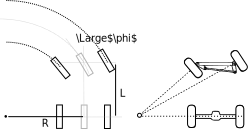
\includegraphics[width=0.9\textwidth]{figs/ackermann.png}
    \def\svgwidth{0.9\textwidth}
    \import{./figs/kinematics/}{swedishwheel.pdf_tex}
    \caption{Omni-directional robot using ``swedish wheels'' in different configurations. Each wheel has two velocity components, speed perpendicular to the wheel's main axis and speed of the rollers. Arrows on the robot body indicate the resulting direction of motion and rotation. }
    \label{fig:swedishwheel}
\end{figure}

Similar to a differential wheel platform, each wheel also imparts a rotation on the robot body. As the wheels are mounted off the center axle, each wheel contributes to two angular moments. One around the horizontal axis with distance $h_i$ to the robot's center, the other around the vertical axis with distance $r_i$ to the robot's center (Figure \ref{fig:swedishwheel}, bottom, center). All combined, the rotation of each wheel will add up to the robot moving with velocities $v_x$, $v_y$ and $\omega_z$.

The velocity at each wheel has two components, the velocity of the $i$-th wheel perpendicular to its main axis $v_{i,m}$, and the velocity of the rollers $v_{i,r}$ that is either $+45\deg$ or $-45\deg$ to the wheel axis. Note that for the system to work, diagonally opposite wheels need to have the same angle. Let the angle of the roller of wheel $i$ be $\gamma_i$. We can now derive the following equations following \cite{maulana2015inverse}:
\begin{equation}\label{eq:swedish1}
v_{i,m}+v_{i,r}\cos(\gamma_i) = v_x - h_i*\omega_z
\end{equation}
That is, the velocity components perpendicular to the wheel axis are equivalent to the forward velocity of the robot plus the velocity component at the wheel resulting from the robot's angular velocity. (Positive angular velocity will result into backward motion per definition of the robot coordinate system.) Similarly, we can write
\begin{equation}\label{eq:swedish2}
v_{i,r}\sin(\gamma_i) = v_y+r_i*\omega_z
\end{equation}
Note that there is no lateral component to the main wheel's motion, as lateral motion can only be achieved via the rollers.

Dividing (\ref{eq:swedish2}) by (\ref{eq:swedish1}) and solving for $v_i$ results into
\begin{equation}
v_i=v_x-h_i\omega_z-\frac{v_y+r_i\omega_z}{\tan{\gamma_i}}
\end{equation}
With $h_i \in h =\{h,-h,h,-h\}$, $r_i \in r=\{r,r,-r,-r\}$ and
$\gamma_i \in \gamma=\{-45\deg,+45\deg,+45\deg,-45\deg\}$ to reflect the different configuration of each wheel, we can derive an expression for the controllable wheel velocities $v_{i,m}$

\begin{eqnarray}
v_{1,m} &=& v_x+v_y+r\omega_z-h\omega_z \\
v_{2,m} &=& v_x-v_y-r\omega_z+h\omega_z \nonumber\\
v_{3,m} &=& v_x-v_y+r\omega_z-h\omega_z \nonumber\\
v_{4,m} &=& v_x+v_y-r\omega_z+h\omega_z \nonumber
\end{eqnarray}

With $v_{i,m}=R\omega_i$ and $R$ the radius of each Swedish wheel, we can now compute the required wheel velocity for any desired robot velocity $v_x$, $v_y$, and $\omega_z$.

\subsection{Feedback control for mobile robots}\label{sec:fbmobile}
\label{sec:kinematics:inverse:feedbackcontrol}

Assume the robot's position to be given by $x_r, y_r$ and $\theta_r$ and the desired pose as $x_g, y_g$ and $\theta_g$---with the subscript $g$ indicating ``goal''.
We can now calculate the error in the desired pose by:
\begin{eqnarray}
\rho  &=& \sqrt{(x_r-x_g)^2+(y_r-y_g)^2} \nonumber \\
\alpha&=& \tan^{-1}{\frac{y_g-y_r}{x_g-x_r}}-\theta_r \\
\eta  &=& \theta_g-\theta_r\ , \nonumber
\end{eqnarray}
which is illustrated in Figure~\ref{fig:trajectorygen}.
These errors can be converted directly into robot's speeds, for example using a simple proportional controller with gains $p_1$, $p_2$ and $p_3$:
\begin{eqnarray}
\dot{x} &=& p_1 \rho\\
\dot{\theta} &=& p_2 \alpha + p_3 \eta
\end{eqnarray}
which will let the robot drive in a curve until it reaches the desired pose.

\begin{figure}
    \centering
    % 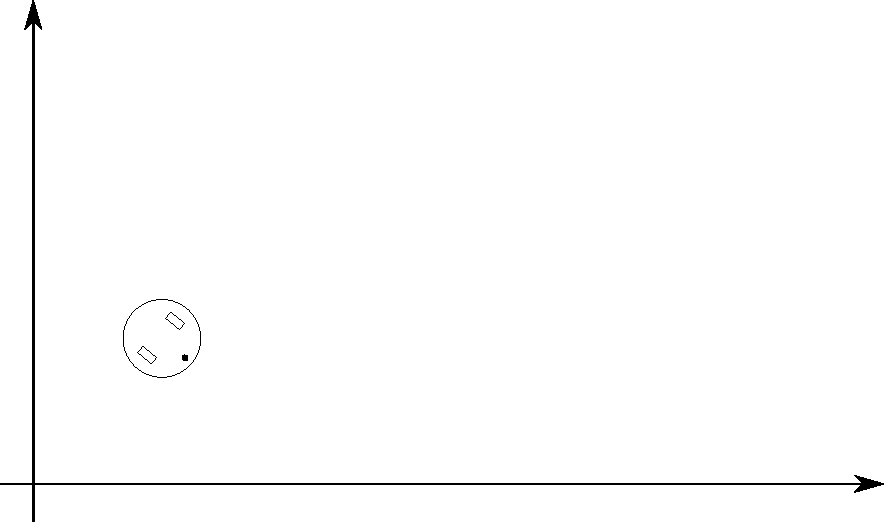
\includegraphics[width=\textwidth]{figs/trajectorygen.png}
    \def\svgwidth{\textwidth}
    \import{./figs/kinematics/}{trajectorygen.pdf_tex}
    \caption{Difference in desired and actual pose as a function of distance $\rho$, bearing $\alpha$ and heading $\eta$.}
    \label{fig:trajectorygen}
\end{figure}


\subsection{Under-actuation and Over-actuation}\label{sec:kinematics:diff:underover}

As detailed at the beginning of this Chapter, kinematics is concerned with analyzing the mapping between our control variables (i.e. the robot's motors represented by the $n$ DoFs in joint space) and their effect on the motion of the robot (our $m$ DoFs in task/configuration space). These two spaces might have different dimensionality, and the relation between these two dimensions greatly affects how we can solve the kinematic problem. It is convenient to analyze these differences by looking at the Jacobian $J$, since the size of the matrix is $m \times n$; in all, we have three different conditions:

\begin{itemize}
\item $n   =  m \rightarrow$ The robot is \textsl{fully actuated}.\index{Fully actuated} The Jacobian $J$ is square and full rank, and the forward kinematics equation is directly invertible;
\item $n \leq m \rightarrow$ The robot is \textsl{under actuated},\index{Under actuated} and the kinematics problem is \textsl{kinematically deficient}. The Jacobian $J$ is ``tall'', because there are more columns $m$ than rows $n$, and not invertible any more; the only way to solve the inverse kinematics problem is through the pseudo-inverse $J^+$ (and similar/more advanced approaches).
\item $n \geq m \rightarrow$ The robot is \textsl{over actuated},\index{Over actuation} and the kinematics problem is \textsl{kinematically redundant}. The Jacobian $J$ is ``fat'', because there are more rows $n$ than columns $m$, and not invertible any more; the only way to solve the inverse kinematics problem is through the pseudo-inverse $J^+$ (and similar/more advanced approaches). In this scenario, it is useful to determine the redundancy coefficient $n-m$ which affects the space of solutions of the inverse kinematic problem.
\end{itemize}

Over- and under-actuation are important design considerations to keep in mind when choosing a robot for a particular task.
In a \textsl{kinematically deficient}\index{Kinematic deficiency} scenario, the robot is not capable of full motion in task space, as it does not have sufficient degrees of freedom in joint space to ``cover'' every possible configuration in task space. This does not mean that the robot is useless! It can still perform tasks---just not \textsl{every} possible task you might ask it to perform.
Conversely, if the problem is \textsl{kinematically redundant},\index{Kinematic redundancy} the robot has more joint DoFs available than it needs, and there exist an infinite number of inverse kinematics solutions in non-singular configurations.
Contrarily to what one may think, redundancy is actually a great feature to have in a robot system, in that it enables flexibility and versatility in solving the kinematic problem: that is, it is possible to choose \textsl{the best} solution among many, and one that satisfies additional constraints and requirements.
% As a matter of fact, the number of inverse kinematics solutions is $\infty^{n-m}$,
A human arm (without considering the hand) is a good example of a kinematically redundant manipulator, as it is equipped with seven DoFs in joint space (three at the shoulder, one at the elbow and three at the wrist), whereas the task space is of dimension six (i.e. the three positions and three orientations of the wrist).
This additional degree of mobility allows humans to reach for objects in multiple configurations, choose motions that are energy efficient, avoid obstacles, and more!


%%%%%%%%%%%%%%%%%%%%

\section*{Take-home lessons}

\begin{itemize}
\item Forward kinematics deals with finding a coordinate transform from a world coordinate system into a coordinate system on the robot.
Such a transform is a combination of a ($3\times1$) translation vector and a ($3\times3$) rotation matrix that consists of the unit vectors of the robot coordinate system. Both translation and rotation can be combined into a $4\times4$ homogeneous transform matrix.
\item Forward and Inverse Kinematics of a mobile robot are performed with respect to the speed of the robot and not its position.
\item To calculate the effect of each wheel on the speed of the robot, you need to consider the contribution of each wheel independently.
%\item You can then plan in configuration space of the robot using path-planning techniques.
\item The inverse kinematics of a robot involves solving the forward kinematics equations for the joint angles.
Calculating the inverse kinematics analytically becomes quickly infeasible, and is impossible for complicated mechanisms.
\item A simple numerical solution is provided by taking all partial derivatives of the forward kinematics in order to get an easily invertible expression that relates joint speeds to end-effector speeds.
\item The inverse kinematics problem can then be formulated as feedback control problem, which will move the end-effector towards its desired pose using small steps. Problems with this approach are local minima and singularities of the mechanism, which might render this solution infeasible.
\item Redundancy allows a robot to solve a kinematic problem in multiple different ways, thus providing better dexterity and versatility in its motion.
\end{itemize}

\section*{Exercises}\small
\subsection*{Coordinate systems}
\begin{enumerate}
\item
\begin{enumerate}
 \item Write out the entries of a rotation matrix $^A_BR$ assuming basis vectors $X_A$, $Y_A$, $Z_A$, and $X_B$, $Y_B$, $Z_B$.
 \item Write out the entries of rotation matrix $^B_AR$.
 \end{enumerate}
\item Assume two coordinate systems that are co-located in the same origin, but rotated around the $z-$axis by the angle $\alpha$. Derive the rotation matrix from one coordinate system into the other and verify that each entry of this matrix is indeed the scalar product of each basis vector of one coordinate system with every other basis vector in the second coordinate system.
\item Consider two coordinate systems $\{B\}$ and $\{C\}$, whose orientation is given by the rotation matrix $^C_BR$ and have distance $^BP$. Provide the homogenous transform $^C_BT$ and its inverse $^B_CT$.
\item Consider the frame $\{B\}$ that is defined with respect to frame $\{A\}$ as $\{B\}=\{^A_BR, ^AP\}$. Provide a homogeneous transform from $\{A\}$ to $\{B\}$.
\item Program a simple application that displays a 2D (or 3D) coordinate system and add the ability to move and turn the coordinate system using your keyboard.
\end{enumerate}

\subsection*{Forward and inverse kinematics}
\begin{enumerate}
\item Consider a differential wheel robot with a broken motor, i.e., one of the wheels cannot be actuated anymore. Derive the forward kinematics of this platform. Assume the right motor is broken.
\item Consider a tri-cycle with two independent standard wheels in the rear and the steerable, driven front-wheel. Choose a suitable coordinate system and use $\phi$ as the steering wheel angle and wheel-speed $\dot{\omega}$. Provide forward and inverse kinematics.
\item Program an application that displays a differential wheel platform and allows you to control forward and rotational speed with your keyboard. Output the robot's pose after every step.
\item Program an application that displays a two-link robotic arm moving in the plane and lets you change both joint angles using your keyboard.
\item Derive the forward kinematics of a two-link robotic arm as well as its Jacobian. Implement its inverse kinematic using the inverse Jacobian technique.
\item Program an application that displays a two-link robotic arm moving in the plane and lets you change the position of its end-effector using your keyboard.
\item Explore the internet for toolkits that allow you to manage forward and inverse kinematics for a robotic arm. What kind of tools do you find and what kind of input do they require to model the robot's geometry?
\item Download the manual of a commercially available robot arm of your choice. What kind of input does it take from its user? Does it allow you to control its position directly?
\item Use a robot simulator of your choice to access a simulated vehicle. What kind of actuator input can you provide and what are the sensors that are available? Drive the car using your keyboard and try to estimate its pose by implementing odometry.
\item Can you provide an example of a kinematically deficient and a kinematically redundant robot manipulator?
\end{enumerate}
\normalsize

